\documentclass{article}

\usepackage{amsmath, amsthm, amssymb, amsfonts}
\usepackage{thmtools}
\usepackage{graphicx}
\usepackage{setspace}
\usepackage{geometry}
\usepackage{float}
\usepackage{hyperref}
\usepackage[utf8]{inputenc}
\usepackage[english]{babel}
\usepackage{framed}
\usepackage[dvipsnames]{xcolor}
\usepackage[most]{tcolorbox}
\usepackage{minted}
\usepackage{enumitem}
\usepackage{booktabs}
\usepackage{multirow}

\usepackage{indentfirst}

\usepackage[export]{adjustbox} % Align images

\colorlet{LightGray}{White!90!Periwinkle}
\colorlet{LightOrange}{Orange!15}
\colorlet{LightGreen}{Green!15}

\newcommand{\HRule}[1]{\rule{\linewidth}{#1}}

\newtcbtheorem[auto counter,number within=section]{code}{Código}{
  colback=LightOrange!20,
  colframe=LightOrange,
  colbacktitle=LightOrange,
  fonttitle=\bfseries\color{black},
  boxed title style={size=small,colframe=LightOrange},
}{code}

\setstretch{1.2}
\geometry{
  textheight=22.5cm,
  textwidth=13.75cm,
  top=2.5cm,
  headheight=12pt,
  headsep=25pt,
  footskip=30pt
}

% ------------------------------------------------------------------------------

\begin{document}

% ------------------------------------------------------------------------------
% Cover Page and ToC
% ------------------------------------------------------------------------------
\begin{center}
  \begin{figure}
    
\includegraphics[scale = 0.3, left]{img/IST_A.eps} % IST logo
    \end{figure}
  \LARGE{ \normalsize \textsc{} \\
  [2.0cm] 
  \LARGE{ \LARGE \textsc{Machine Learning}} \\
  [1cm]
  \LARGE{ \LARGE \textsc{LEIC IST-UL}} \\
  [1cm]
  \HRule{1.5pt} \\
  [0.4cm]
  \LARGE \textbf{\uppercase{Relatório - Homework 1}}
  \HRule{1.5pt}
  \\ [2.5cm]
  }
\end{center}

\begin{flushleft}
  \textbf{\LARGE Grupo 10:}
\end{flushleft}

\begin{center}
  \begin{minipage}{0.7\textwidth}
      \begin{flushleft}
        \large Gabriel Ferreira \\
        \large  Irell Zane
      \end{flushleft}
  \end{minipage}%
  \begin{minipage}{0.3\textwidth}
      \begin{flushright}
        \large 107030\\
        \large 107161
      \end{flushright}
  \end{minipage}
\end{center}

\begin{center}
  \vspace{4cm}
  \date \large \bf  2024/2025 -- 1st Semester, P1
\end{center}

\setcounter{page}{0}
\thispagestyle{empty}
\renewcommand{\thesection}{\Roman{section}}

\newpage

% ------------------------------------------------------------------------------
% Content
% ------------------------------------------------------------------------------



\large{\textbf{Part I}: Pen and paper}\normalsize




\begin{enumerate}[leftmargin=\labelsep]
\item Completion of the decision tree.

\hspace{3pt}

\begin{minipage}{0.4\textwidth}
  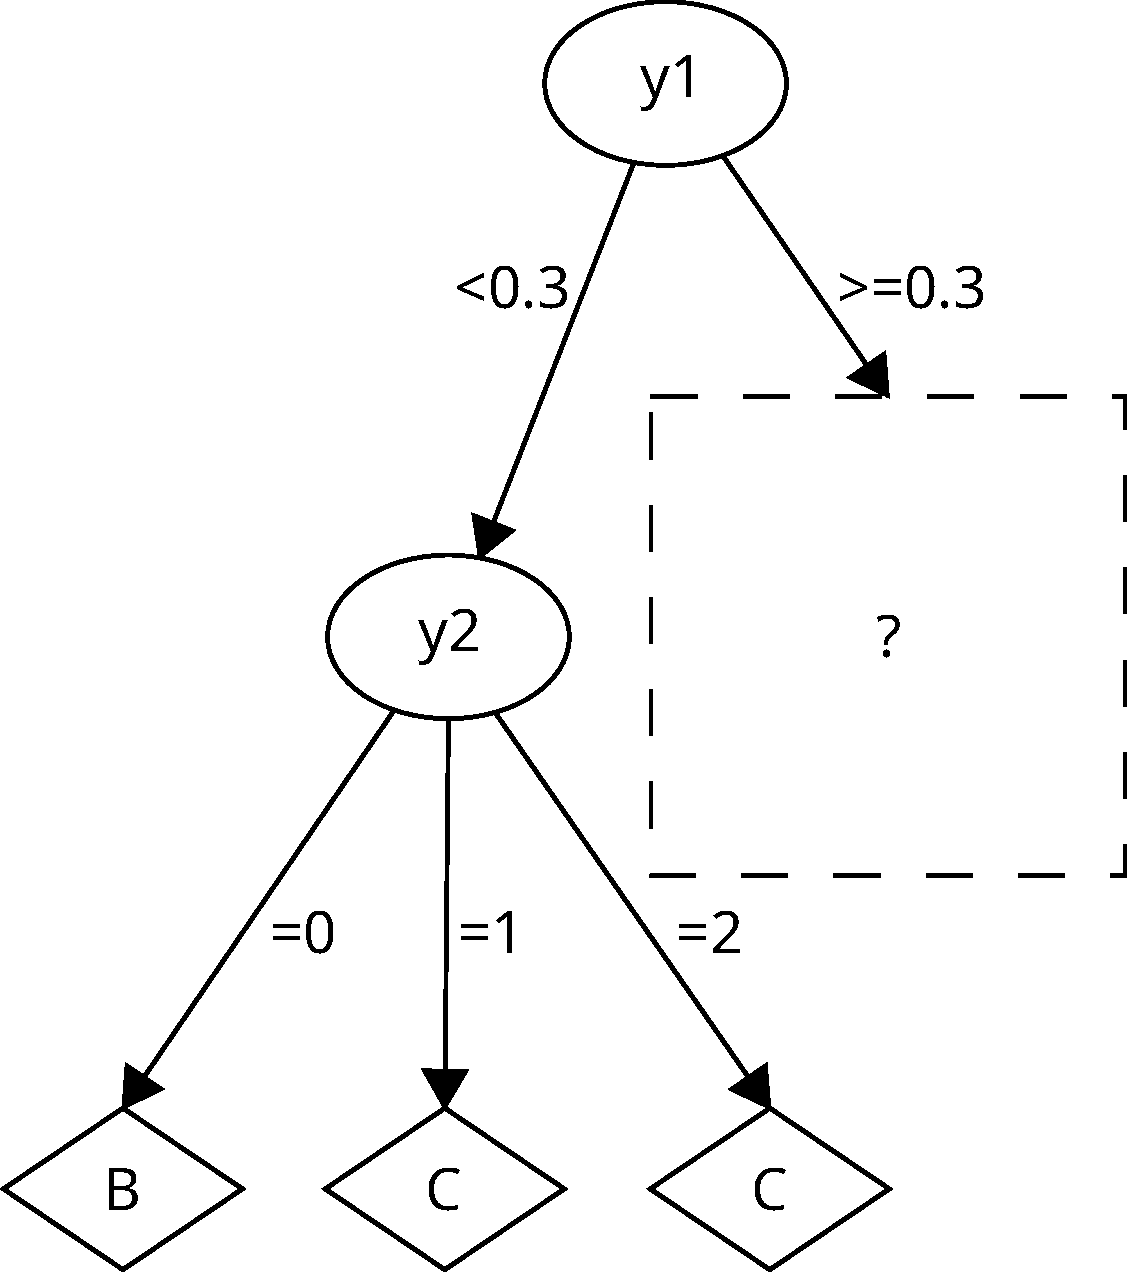
\includegraphics[scale = 0.3, left]{img/decision_tree_1.pdf}
\end{minipage}
\hspace{0.05\textwidth}
\begin{minipage}{0.6\textwidth}
  The node we must decide what to do it is on the right for 
  the dataset $D | (y1 >= 0.3)$.
  \begin{table}[H]
    \centering
    \begin{tabular}{@{}ccccc}
      $D | (y1 >= 0.3)$ & $y_2$ & $y_3$ & $y_4$ & $y_{out}$ \\ \midrule
      $x_6$  & 0 & 1 & 0 & B \\
      $x_7$  & 0 & 1 & 1 & A \\
      $x_8$  & 1 & 0 & 0 & A \\
      $x_9$  & 0 & 1 & 1 & C \\
      $x_{10}$ & 0 & 1 & 1 & C \\
      $x_{11}$ & 1 & 0 & 0 & A \\
      $x_{12}$ & 1 & 2 & 0 & B \\
    \end{tabular}
  \end{table}

  Since there are distinct $y_{out}$ values, and more 
  than 4 observations. We can split this node.
\end{minipage}
 
\hspace{3pt}

To decide the next variable to use, we must calculate 
the Information Gain of each variable using Shannon 
entropy for the dataset.

\begin{equation*}
    H(y_{out}) = -\frac{3}{7}log_2(\frac{3}{7})-\frac{2}{7}log_2(\frac{2}{7})-\frac{2}{7}log_2(\frac{2}{7}) \\ [2ex]
    = 1.57
\end{equation*}

\begin{equation*}
  H(y_{out}|y_j) = \sum{-p log_2}
\end{equation*}

\begin{equation*}
  IG(y_j) = H(y_{out}) - H(y_{out}|y_j)
\end{equation*}

\begin{table}[H]
  \begin{tabular}{cc|ccccc|cc}
  $j$ & $x$                    & $p(x)$        & $p(A | x)$   & $p(B | x)$   & $p(C | x)$   & $H(y_{out}|x)$ & $H(y_{out}|y_j)$ & $IG(y_{out}|y_j)$ \\ \midrule
  \multirow{2}{*}{2} & $y_2=0$ & $\frac{4}{7}$ & $\frac{1}{4}$ & $\frac{1}{4}$ & $\frac{2}{4}$ & 1.5  & \multirow{2}{*}{1.25} & \multirow{2}{*}{0.31} \\
   &                   $y_2=1$ & $\frac{3}{7}$ & $\frac{2}{3}$ & $\frac{1}{3}$ & $\frac{0}{3}$ & 0.92 &  &  \\ \midrule
  \multirow{3}{*}{3} & $y_3=0$ & $\frac{2}{7}$ & $\frac{2}{2}$ & $\frac{0}{2}$ & $\frac{0}{2}$ & 0    & \multirow{3}{*}{0.86} & \multirow{3}{*}{0.70} \\
   &                   $y_3=1$ & $\frac{4}{7}$ & $\frac{1}{4}$ & $\frac{1}{4}$ & $\frac{2}{4}$ & 1.5  &  &  \\
   &                   $y_3=2$ & $\frac{1}{7}$ & $\frac{0}{1}$ & $\frac{1}{1}$ & $\frac{0}{1}$ & 0    &  &  \\ \midrule
  \multirow{2}{*}{4} & $y_4=0$ & $\frac{4}{7}$ & $\frac{2}{4}$ & $\frac{2}{4}$ & $\frac{0}{4}$ & 1    & \multirow{2}{*}{0.96} & \multirow{2}{*}{0.60} \\
   &                   $y_2=4$ & $\frac{3}{7}$ & $\frac{1}{3}$ & $\frac{0}{3}$ & $\frac{2}{3}$ & 0.92 &  &  \\ \bottomrule
  \end{tabular}
\end{table}

Seeing that $y_4$ is the variable with the most information 
gain, it is the one that should be chosen to split the node.


\begin{minipage}{0.5\textwidth}
  \begin{table}[H]
    \centering
    \begin{tabular}{@{}cccc}
      $D | (y1 >= 0.3)$ & $y_2$ & $y_3$ & $y_{out}$ \\ \midrule
      $x_6$    & 0 & 1 & B \\
      $x_8$    & 1 & 0 & A \\
      $x_{11}$ & 1 & 0 & A \\
      $x_{12}$ & 1 & 2 & B \\
    \end{tabular}
  \end{table}
\end{minipage}
\begin{minipage}{0.5\textwidth}
  \begin{table}[H]
    \centering
    \begin{tabular}{@{}cccc}
      $D | (y1 >= 0.3)$ & $y_2$ & $y_3$ & $y_{out}$ \\ \midrule
      $x_7$    & 0 & 1 & A \\
      $x_9$    & 0 & 1 & C \\
      $x_{10}$ & 0 & 1 & C \\
    \end{tabular}
  \end{table}
\end{minipage}

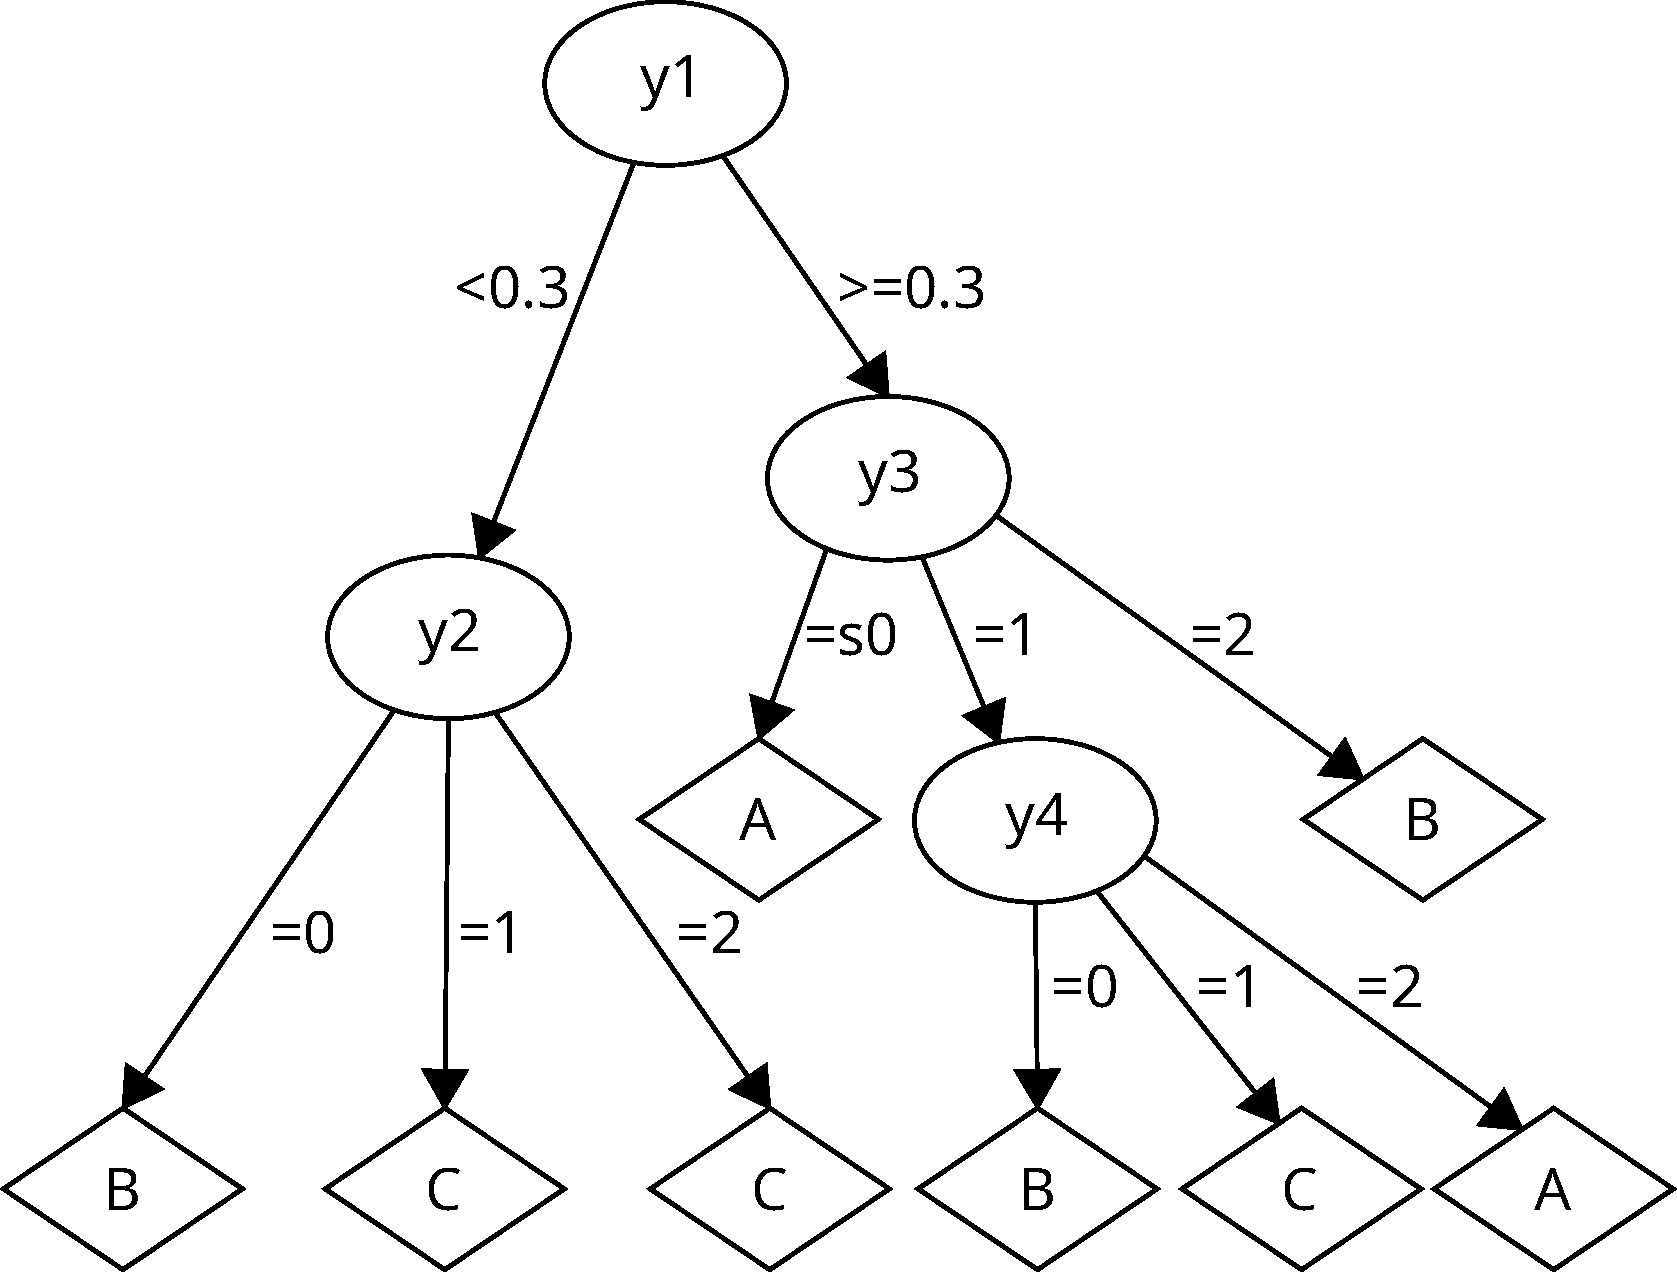
\includegraphics[scale = 0.3, left]{img/decision_tree_3.pdf}


\item Draw the confusion Matrix.


\begin{table}[H]
  \centering
  \begin{tabular}{ccccc}
      & A & B & C & \\ \midrule
    A & &&& \\
    B & &&& \\
    C & &&& \\
  \end{tabular}
\end{table}


\begin{enumerate}
\item Place your solution. Math can be entered using the equation
environment like this
\begin{equation}
    \vec{\mathbf{r}} = \vec{\mathbf{r}}_{0} + \vec{\mathbf{v}}_{0}t + \frac{1}{2}\vec{\mathbf{a}}t^{2}
\end{equation}
If you then where working in say the $x$-direction and had some numbers % A percent sign allows you to comment.
%The dollar signs around something in a line of text is for "in-line math"
\begin{equation}
\begin{array}{r@{~=~}l}
x & x_{0} + v_{x0}t + \frac{1}{2}a_{x}t^{2} \\ [2ex]
& 1.2~\text{m} + (4.0~\text{m/s})(3.0~\text{s}) + \frac{1}{2}(-1.0~\text{m/s}^{2})(3.0~\text{s})^{2}\\ [2ex]
& \boxed{8.7~\text{m}}
\end{array}
\end{equation}

\item When you get to the next part, you can add a \verb"\item" to get the appropriate label. Also,
if you don't like all the equation numbers, you can use the following to have the equation with
no number
\begin{equation*}
\sum\vec{\mathbf{F}} = m\vec{\mathbf{a}}
\end{equation*}

\item For more details on putting math into {\LaTeX} documents you can see 
\href{https://www.overleaf.com/learn/latex/Mathematical_expressions}{this page on Overleaf}.
\end{enumerate}

\item We you get to the next problem, you can end the enumerate for the parts of the previous problem and then add another item.
    \begin{enumerate}
    \item Use a nested enumerate environment to label the parts of the next problem.
    \item For a quick and broad overview of how to create documents in {\LaTeX} see 
    \href{https://www.overleaf.com/learn/latex/Learn_LaTeX_in_30_minutes}{this quick tutorial from Overleaf}.
    \end{enumerate}
\end{enumerate}

\large{\textbf{Part II}: Programming}\normalsize

\begin{enumerate}[leftmargin=\labelsep]
\item Solution to the programming questions here.
\end{enumerate}

\vskip 1cm
\textbf{End note}: do not forget to also submit your Jupyter notebook

\newpage

% ----------------------------------------------------------------------
% Cover
% ----------------------------------------------------------------------

\end{document}
